\documentclass{MMCStyle}
\usepackage{zhlipsum,mwe}
\bianhao{123456}
\tihao{ABCDEFGHI}
\timu{论文标题}
\keyword{content;content;content}
\bibliographystyle{gbt7714-numerical}
\begin{document}
	\begin{abstract}
		Mathorcup\cite{石润2014我国区域金融风险的防范与化解策略研究} Overleaf 模版\cite{AAAAAA}。
        
	%	本模板
	%	\begin{itemize}
	%		\item 定义了几个宏 \lstinline|\def\ee{\mathrm{e}},\def\ii{\mathrm{i}},\def\leq{\leqslant},\def\geq{\geqslant}| 方便使用;
	%		\item 图片应放在 \lstinline|figure| 文件夹中;
	%		\item 定制了 matlab 和 python 代码环境,使用方法:\lstinline|\begin{matlab} content \end{matlab}| 和 \lstinline|\begin{python} content \end{python}|;
	%		\item 加载了 \lstinline|cleveref| 宏包,使用方法:\lstinline|\cref{label}|。
	%	\end{itemize}
	%	其它的就是跟普通的 \lstinline|ctexart| 使用方法一样。
 
        摘要摘要摘要摘要摘要摘要摘要摘要摘要摘要摘要摘要摘要摘要摘要摘要摘要摘要摘要摘要摘要摘要摘要摘要摘要摘要摘要摘要摘要摘要摘要摘要摘要摘要摘要摘要摘要摘要摘要摘要摘要摘要摘要摘要摘要摘要摘要摘要摘要摘要摘要摘要摘要摘要摘要摘要摘要摘要摘要摘要摘要摘要摘要摘要摘要摘要摘要摘要摘要摘要摘要摘要摘要摘要摘要摘要摘要摘要摘要摘要摘要摘要摘要摘要摘要摘要摘要摘要摘要摘要摘要摘要摘要摘要摘要摘要摘要摘要摘要摘要摘要摘要摘要摘要摘要摘要摘要摘要摘要摘要摘要摘要摘要摘要摘要摘要摘要摘要摘要摘要摘要摘要摘要摘要摘要摘要摘要摘要。
        
        摘要摘要摘要摘要摘要摘要摘要摘要摘要摘要摘要摘要摘要摘要摘要摘要摘要摘要摘要摘要摘要摘要摘要摘要摘要摘要摘要摘要摘要摘要摘要摘要摘要摘要摘要摘要摘要摘要摘要摘要摘要摘要摘摘要摘要摘要摘要摘要摘要摘要摘要摘要摘要摘要摘要摘要摘要摘要摘要摘要摘要摘摘要摘要摘要摘要摘要摘要摘要摘要摘要摘要摘要摘要摘要摘要摘要摘要摘要摘要摘要摘要摘要摘要摘要摘要摘要摘要摘要摘要摘要摘要摘要摘要摘要摘要摘要摘要摘要摘要摘要摘要摘要摘要摘要摘要摘要摘要摘要摘要摘要摘要摘要摘要摘要摘要摘要摘要摘要摘要摘要摘要摘要摘要摘要摘要摘要摘要摘要摘要摘要摘要摘要摘要摘要摘要摘要摘要摘要摘要摘要摘要摘要摘要。

        摘要摘要摘要摘要摘要摘要摘要摘要摘要摘要摘要摘要摘要摘要摘要摘要摘要摘要摘要摘要摘要摘要摘要摘要摘要摘要摘要摘要摘要摘要摘要摘要摘要摘要摘要摘要摘要摘要摘要摘要摘要摘要摘要摘要摘要摘要摘要摘要摘要摘要摘要摘要摘要摘要摘要摘要摘要摘要摘要摘要摘要摘要摘要摘要摘要摘要摘要摘要摘要摘要摘要摘要摘要摘要摘要摘要摘要摘要摘要摘要摘要摘要摘要摘要摘要摘要摘要摘要摘要摘要摘要摘要摘要摘要摘要摘要摘要摘要摘要摘要摘要摘要摘要摘要摘要摘要摘要摘要摘要摘要摘要摘要摘要摘要摘要摘要摘要摘要摘要摘要摘要摘要摘要摘要摘要摘要摘要摘要摘要摘要摘要摘要摘要摘要摘要摘要摘要摘要摘要摘要摘要摘要摘要。
	\end{abstract}
	\tableofcontents\newpage
 
	\section{问题的提出}
问题的\cite{石润2023基于}提出问题的提出问题的提出问题的提出问题的提出问题的提出问题的提出问题的提出问题的提出问题的提出问题的提出问题的提出问题的提出问题的提出问题的提出问题的提出问题的提出问题的提出问题的提\cite{石润2023凤仙花种子包衣载体固定化微生物修复石油烃污染土壤的效应}出问题的提出问题的提出问题的提出问题的提出问题的提出问题的提出问题的提出问题的提出问题的提出问题\cite{李韵诗2015重金属污染土壤植物修复中的微生物功能研究进展}的提出问题\cite{AAAAAA}的提出问题的提出。
 
 问题的提出问题的提出问题的提出问题的提出问题的提出问题的提出问题的提出问题的提出问题的提出问题的提出问题的提出问题的提出问题的提出问题的提出问题的提出问题的提出问题的提出问题的提出问题的提出问题的提出问题的提出问题的提出问题的提出问题的提出问题的提出问题的提出问题的提出问题的提出问题的提出问题的提出问题的提出。
 
 问题的提出问题的提出问题的提出问题的提出问题的提出问题的提出问题的提出问题的提出问题的提出问题的提出问题的提出问题的提出问题的提出问题的提出问题的提出问题的提出问题的提出问题的提出问题的提出问题的提出问题的提出问题的提出问题的提出问题的提出问题的提出问题的提出问题的提出问题的提出问题的提出问题的提出问题的提出。问题的提出问题的提出问题的提出问题的提出问题的提出问题的提出问题的提出问题的提出问题的提出问题的提出问题的提出问题的提出问题的提出问题的提出问题的提出问题的提出问题的提出问题的提出问题的提出问题的提出问题的提出问题的提出问题的提出问题的提出问题的提出问题的提出问题的提出问题的提出问题的提出问题的提出问题的提出。
 
	\subsection{问题的背景}
问题的背景问题的背景问题的背景问题的背景问题的背景问题的背景问题的背景问题的背景问题的背景问题的背景问题的背景问题的背景问题的背景问题的背景问题的背景问题的背景问题的背景问题的背景问题的背景问题的背景。

问题的背景问题的背景问题的背景问题的背景问题的背景问题的背景问题的背景问题的背景问题的背景问题的背景问题的背景问题的背景问题的背景问题的背景问题的背景问题的背景问题的背景问题的背景问题的背景问题的背景。问题的背景问题的背景问题的背景问题的背景问题的背景问题的背景问题的背景问题的背景问题的背景问题的背景问题的背景问题的背景问题的背景问题的背景问题的背景问题的背景问题的背景问题的背景问题的背景问题的背景。

问题的背景问题的背景问题的背景问题的背景问题的背景问题的背景问题的背景问题的背景问题的背景问题的背景问题的背景问题的背景问题的背景问题的背景问题的背景问题的背景问题的背景问题的背景问题的背景问题的背景。
	\subsection{问题的提出}
问题的提出问题的提出问题的提出问题的提出问题的提出。问题的提出问题的提出问题的提出问题的提出问题的提出问题的提出问题的提出。

问题的提出问题的提出问题的提出问题的提出问题的提出问题的提出问题的提出问题的提出问题的提出问题的提出问题的提出问题的提出问题的提出问题的提出问题的提出问题的提出问题的提出问题的提出问题的提出问题的提出问题的提出问题的提出问题的提出问题的提出问题的提出问题的提出问题的提出问题的提出问题的提出。

	\section{问题的分析}
问题的分析。问题的分析问题的分析问题的分析问题的分析问题的分析问题的分析问题的分析问题的分析问题的分析问题的分析问题的分析问题的分析问题的分析问题的分析问题的分析问题的分析问题的分析问题的分析问题的分析问题的分析问题的分析问题的分析问题的分析问题的分析问题的分析问题的分析问题的分析问题的分析问题的分析问题的分析问题的分析问题的分析问题的分析问题的分析问题的分析问题的分析问题的分析问题的分析。

问题的分析问题的分析问题的分析问题的分析问题的分析问题的分析问题的分析问题的分析问题的分析问题的分析问题的分析问题的分析问题的分析问题的分析问题的分析问题的分析问题的分析问题的分析问题的分析问题的分析问题的分析问题的分析问题的分析问题的分析问题的分析问题的分析问题的分析问题的分析问题的分析。

	\subsection{问题的整体分析}
问题的整体分析。问题的整体分析。问题的整体分析。问题的整体分析问题的整体分析问题的整体分析问问题的整体分析问题的整体分析问题的整体分析问题的整体分析问题的整体分析问题的整体分析问题的整体分析。

问题的整体分析问题的整体分析问题的整体分析问题的整体分析问题的整体分析问题的整体分析问题的整体分析问题的整体分析问题的整体分析问题的整体分析问题的整体分析。
	\subsection{问题一的分析}
问题一的分析问题一的分析问题一的分析问题一的分析问题一的分析问题一的分析问题一的分析问题一的分析问题一的分析问题一的分析问题一的分析问题一的分析问题一的分析问题一的分析问题一的分析问题一的分析问题一的分析问题一的分析问题一的分析。
	\subsection{问题二的分析}
问题二的分析。问题二的分析问题二的分析问题二的分析问题二的分析问题二的分析问题二的分析问题二的分析问题二的分析问题二的分析问题二的分析问题二的分析问题二的分析问题二的分析问题二的分析问题二的分析问题二的分析。
	\subsection{问题三的分析}
问题三的分析。问题三的分析问题三的分析问题三的分析问题三的分析问题三的分析问题三的分析问题三的分析问题三的分析问题三的分析问题三的分析问题三的分析问题三的分析问题三的分析问题三的分析问题三的分析问题三的分析问题三的分析问题三的分析问题三的分析。

	\section{模型的假设}
	\begin{enumerate}
		\item 假设1;
		\item 假设2;
		\item 假设3;
		\item 假设4;
		\item 假设5
	\end{enumerate}
	\section{符号说明}
	\begin{center}
		\begin{tabularx}{0.7\textwidth}{c@{\hspace{1pc}}|@{\hspace{2pc}}X}
			\Xhline{0.08em}
			符号 & \multicolumn{1}{c}{符号说明}\\
			\Xhline{0.05em}
			$\delta$ & 符号1\\
			$\beta$ & 符号2\\
			$\alpha$ & 符号3\\
			$r$ & 符号4\\
			$\gamma$ & 符号5\\
			$l$ & 符号6\\
			$l_{y}$ & 符号7\\
			$\vec{x}_{1},\vec{y}_{1},\vec{z}_{1}$ & 符号8\\
			$\vec{\hat{x}}_{1},\vec{\hat{y}}_{1},\vec{\hat{z}}_{1}$ & 符号9\\
			$\theta$ & 符号10\\
			$l_{y}(i)$ & 编号为 $i$ 符号11\\
			$\theta_{i}$ & 编号为 $i$ 符号12\\
			\Xhline{0.08em}
		\end{tabularx}
	\end{center}

	\section{模型的建立与求解}
模型的建立与求解模型的建立与求解模型的建立与求解模型的建立与求解模型的建立与求解模型的建立与求解模型的的建立与求解模型的建立与求解模型的建立与求解模型的建立与求解模型的建立与求解模型的建立与求解模型的建立与求解模型的建立与求解模型的建立与求解模型的建立与求解模型的建立与求解模型的建立与求解模型的建立与求解。

模型的建立与求解模型的建立与求解模型的建立与求解模型的建立与求解模型的建立与求解模型的建立与求解模型的建立与求解模型的建立与求解模型的建立与求解模型的建立与求解模型的建立与求解模型的建立与求解模型的建立与求解模型的建立与求解模型的建立与求解。
	\subsection{模型的准备}
模型的准备模型的准备模型的准备模型的准备模型的准备模型的准备模型的准备模型的准备模型的准备模型的准备模型的准备模型的准备。模型的准备模型的准备模型的准备模型的准备模型的准备模型的准备模型的准备模型的准备模型的准备模型的准备模型的准备模型的准备模型的准备。

模型的准备模型的准备模型的准备模型的准备模型的准备模型的准备模型的准备模型的准备模型的准备模型的准备模型的准备模型的准备模型的准备。

	\subsection{模型一的建立}
 模型一的建立模型一的建立模型一的建立模型一的建立模型一的建立模型一的建立模型一的建立模型一的建立模型一的建立模型一的建立模型一的建立模型一的建立模型一的建立模型一的建立模型一的建立模型一的建立模型一的建立模型一的建立模型一的建立模型一的建立模型一的建立模型一的建立模型一的建立模型一的建立模型一的建立。
	效果见\cref{fig:1}。
	\begin{figure}[h]
		\centering
		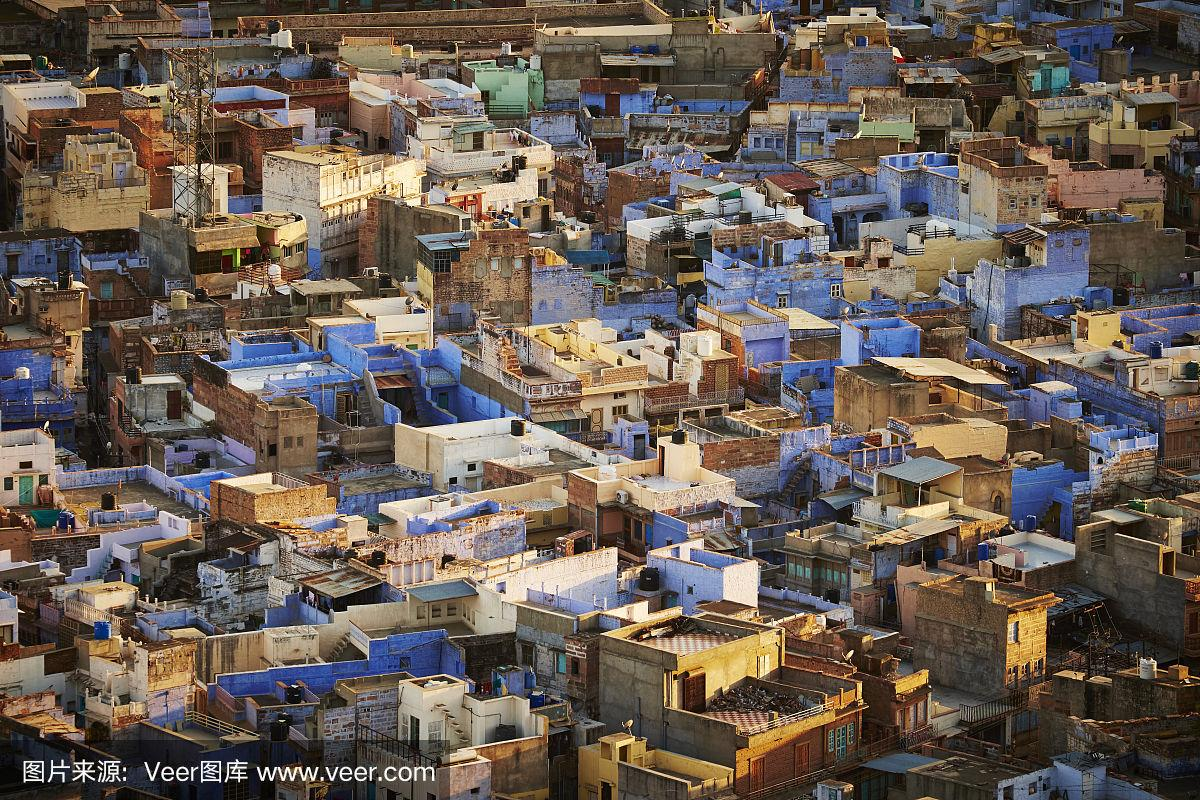
\includegraphics[width=0.4\textwidth]{figure/image.png}
		\caption{content}\label{fig:1}
	\end{figure}
 模型一的建立模型一的建立模型一的建立模型一的建立模型一的建立模型一的建立模型一的建立模型一的建立模型一的建立模型一的建立模型一的建立模型一的建立模型一的建立模型一的建立模型一的建立模型一的建立模型一的建立。

 模型一的建立模型一的建立模型一的建立模型一的建立模型一的建立模型一的建立模型一的建立模型一的建立模型一的建立模型一的建立模型一的建立模型一的建立。模型一的建立。
	\subsection{模型二的建立}
 
	结果见\cref{tab:1}。
 
	\begin{table}[h]
		\centering
		\caption{content}\label{tab:1}
		\begin{tabularx}{0.7\textwidth}{c@{\hspace{1pc}}|@{\hspace{2pc}}X}
		\Xhline{0.08em}
		符号 & \multicolumn{1}{c}{符号说明}\\
		\Xhline{0.05em}
		$\delta$ & 赤纬角\\
		$\beta$ & 经度\\
		$\alpha$ & 纬度\\
		$r$ & 地球半径\\
		$\gamma$ & 太阳光与杆所成的夹角\\
		$l$ & 杆的长度\\
		$l_{y}$ & 杆的影子长度\\
		$\vec{x}_{1},\vec{y}_{1},\vec{z}_{1}$ & 由杆的位置所生成的切平面的正交基\\
		$\vec{\hat{x}}_{1},\vec{\hat{y}}_{1},\vec{\hat{z}}_{1}$ & 由杆的位置所生成的切平面的单位正交基\\
		$\theta$ & 影子与北方的夹角\\
		$l_{y}(i)$ & 编号为 $i$ 的数据对应的影子长度\\
		$\theta_{i}$ & 编号为 $i$ 的数据对应的影子角度\\			\Xhline{0.08em}
		\end{tabularx}
	\end{table}
 
	\subsection{模型三的建立}
	模型三的建立模型三的建立模型三的建立模型三的建立模型三的建立模型三的建立模型三的建立模型三的建立模型三的建立模型三的建立模型三的建立模型三的建立模型三的建立模型三的建立模型三的建立模型三的建立模型三的建立模型三的建立模型三的建立模型三的建立模型三的建立模型三的建立。

	\section{模型的检验}
	模型的检验模型的检验模型的检验模型的检验模型的检验模型的检验模型的检验模型的检验模型的检验模型的检验模型的检验模型的检验模型的检验模型的检验模型的检验模型的检验模型的检验模型的检验模型的检验模型的检验模型的检验模型的检验模型的检验。

	\section{模型的评价与改进}
	模型的评价与改进模型的评价与改进模型的评价与改进模型的评价与改进模型的评价与改进模型的评价与改进模型的评价与改进模型的评价与改进模型的评价与改进模型的评价与改进模型的评价与改进模型的评价与改进模型的评价与改进模型的评价与改进模型的评价与改进模型的评价与改进模型的评价与改进模型的评价与改进。
 
	\subsection{模型的优点}
	模型的优点。模型的优点模型的优点模型的优点模型的优点模型的优点模型的优点模型的优点模型的优点模型的优点模型的优点模型的优点模型的优点模型的优点模型的优点模型的优点。
	\subsection{模型的缺点}
	模型的缺点。模型的缺点模型的缺点模型的缺点模型的缺点模型的缺点模型的缺点模型的缺点模型的缺点模型的缺点模型的缺点模型的缺点模型的缺点模型的缺点模型的缺点模型的缺点模型的缺点模型的缺点模型的缺点模型的缺点。
	\subsection{模型的改进}
	模型的改进。模型的改进模型的改进模型的改进模型的改进模型的改进模型的改进模型的改进模型的改进模型的改进模型的改进模型的改进模型的改进模型的改进模型的改进模型的改进模型的改进模型的改进模型的改进模型的改进模型的改进模型的改进模型的改进模型的改进模型的改进模型的改进模型的改进模型的改进。

	\phantomsection
	\addcontentsline{toc}{section}{参考文献}
	\bibliography{ref}

	\newpage
	\appendix
	\ctexset{section={
		format={\zihao{-4}\heiti\raggedright}
	}}
	\begin{center}
		\heiti\zihao{4} 附\hspace{1pc}录
	\end{center}
	\section{问题一的 MATLAB 代码}
	
 \begin{matlab}
    clc,clear
    %第七题
    R71 = 1;
    R72 = 2;
    T7 = 1;
    K7 = 1;
    N7=10^5;
    G71=tf(R72,R71);
    G72=tf(1,[T7 1]);
    G73=tf(1,[T7 0]);
    G74=tf([N7*T7 0],[T7 N7]);
    G75=tf([N7*K7*T7 N7*K7],[T7 N7]);
    G76=tf([K7*T7 K7],[T7 0]);
    
    subplot(2,3,1)
    step(G71)
    xlabel('$t$','interpreter','latex', 'FontSize', 12);
    ylabel('$y$','interpreter','latex', 'FontSize', 12);
    title('比例环节');
	
 \end{matlab}
 \section{问题一的 python 代码}
  \begin{python}
      import torch
      import numpy as np
      import pandas as pd
      for i in range(100):
          print('demo')
  \end{python}
\end{document}